\documentclass{beamer}

% Top-aligning columns within a top-aligned frame
% https://tex.stackexchange.com/questions/16447/beamer-top-aligning-columns-within-a-top-aligned-frame
\makeatletter
\newenvironment{myitemize}{%
   \setlength{\topsep}{0pt}
   \setlength{\partopsep}{0pt}
   \renewcommand*{\@listi}{\leftmargin\leftmargini \parsep\z@ \topsep\z@ \itemsep\z@}
   \let\@listI\@listi
   \itemize
}{\enditemize}
\makeatother  

\usepackage[USenglish]{babel}
\usepackage[utf8]{inputenc}
\usepackage{amssymb, amsmath}
\usepackage{bm}
\usepackage{color}
\usepackage{tikz}
\usepackage{url}

\definecolor{links}{HTML}{2A1B81}
\hypersetup{colorlinks,linkcolor=,urlcolor=links}

\usetheme{Boadilla}

\bibliographystyle{apalike}
% make bibliography entries smaller
%\renewcommand\bibfont{\scriptsize}
% Now get rid of all the colours
\setbeamercolor*{bibliography entry title}{fg=black}
\setbeamercolor*{bibliography entry author}{fg=black}
\setbeamercolor*{bibliography entry location}{fg=black}
\setbeamercolor*{bibliography entry note}{fg=black}

\newcommand{\lnorm}[1]{\left\lVert#1\right\rVert^2}
\newcommand{\norm}[1]{\left\lVert#1\right\rVert}

% and kill the abominable icon
\setbeamertemplate{bibliography item}{}

\begin{document}
\title[NBDT]{NBDT: Neural-Backed Decision Trees}  
\author{Radek Bartyzal}
\date{5. 5. 2020} 
\institute{GLAMI AI}

\frame{\titlepage} 

\begin{frame}{Motivation}

Interpretability of models:
\begin{itemize}
\item decision trees = good
\item neural nets = bad
\end{itemize}

\vfill

Saliency maps:
\begin{itemize}
\item tells you what the nets is "looking" at
\item good for debugging = is the net focusing on the right object?
\item does not help if the net looks at the right object but predicts wrong class
\end{itemize}

\end{frame}

%--------- END Frame 12 -------------


%--------- END Frame 12 -------------
\begin{frame}{Overview}

\begin{figure}[h]
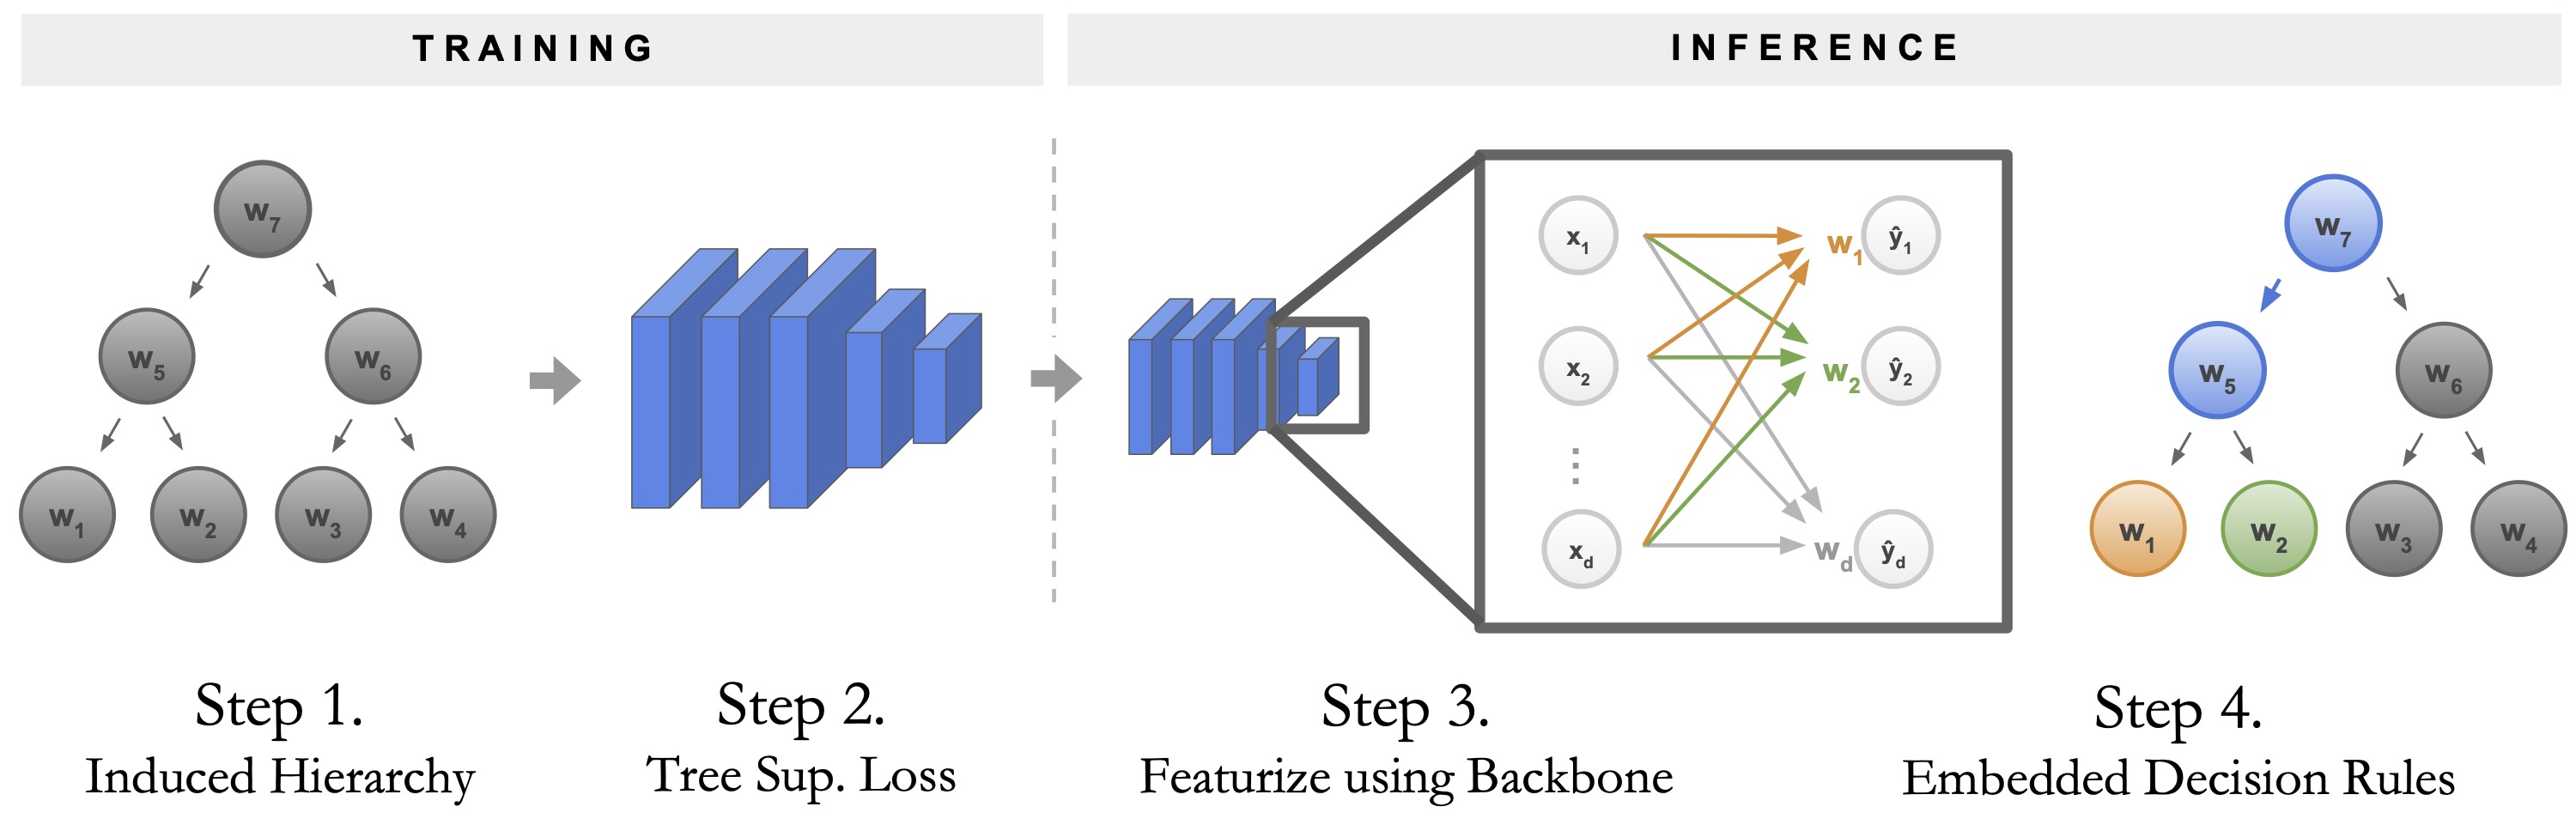
\includegraphics[width=\textwidth]{img/train}
\caption{}
\end{figure}

\end{frame}

%--------- END Frame 12 -------------
\begin{frame}{Prediction}

\begin{itemize}
\item get embedding of the sample = $x$ = output of the pre-last layer
\item take the last weight matrix $W$ of the net = the producing the prediction probabilities
\item each row $w_i$ corresponds to one output = class
\item each class $c$ = leaf node $c$ => $w_c$ = $r_c$ = representation vector of node $c$  
\item probability of node $n$ = $<xr_n^T>$ = for leaf node $c$ = $xw_c^T$
\item representation vector of inner node = average of repr. vectors of child nodes
\end{itemize}

\end{frame}
%--------- END Frame 12 -------------
\begin{frame}{Training}

\begin{itemize}
\item pre-train the model on the dataset
\item construct the nodes by hierarchical clustering done from the $w_i$ rows of the final weight matrix = get hierarchy of nodes = decision tree
\item fine-tune the model on the fixed hierarchy to cluster the $w_i$ of the parent nodes together better
\end{itemize}

\end{frame}

%--------- END Frame 12 -------------

\begin{frame}{Sources}

\begin{thebibliography}{0}

  \bibitem[1]{cit:paper} 1. Wan, Alvin, et al. "NBDT: Neural-Backed Decision Trees." arXiv preprint arXiv:2004.00221 (2020). \url{https://arxiv.org/abs/2004.00221} 
  
  \bibitem[2]{cit:blog} 2. Blog post with links to code. \url{https://bair.berkeley.edu/blog/2020/04/23/decisions/}
  
\end{thebibliography}

\end{frame}

 
\end{document}
